\begin{table}
\caption{Overview of assimilation experiments performed.}
\centering
\begin{tabular}{p{2cm}p{2cm}p{6cm}p{4cm}}
	Experiment& Model &  Assimilated Quantities  & Run dates \\
\hline
E1 & WACCM &	none   & 1 Oct 2009 - 31 Mar 2010	\\
E2 & WACCM &	GPS-RO + NNRA$^a$ tropics only & 1 Oct 2009 - 31 Mar 2010	\\
E3 & WACCM &	GPS-RO + NNRA$^a$ whole atmosphere  & 1 Oct 2009 - 31 Mar 2010	\\
E4 & CAM	&	none &  1 Jan - 28 Feb 2009 \\
E5 & CAM &	$\chi_1$, $\chi_2$, $\Delta$LOD	& 1 Jan - 28 Feb 2009 \\
E6 & CAM &	Temperature	& 1 Jan -31 Jan 2009	\\
E7 & CAM &	Temperature, $\chi_1$, $\chi_2$, $\Delta$LOD	& 1 Jan - 17 Jan 2009\\
\hline
\end{tabular}
\tablenotetext{a}{Observations used in the NCEP/NCAR Reanalysis project \citet{Saha2010}, which include radiosonde and aircraft winds and temperatures, plus satellite drift winds.}
\label{tab:expts}
\end{table}
\clearpage

%-------comparison of the WACCM experiments in terms of true error ----
 \begin{figure}
	 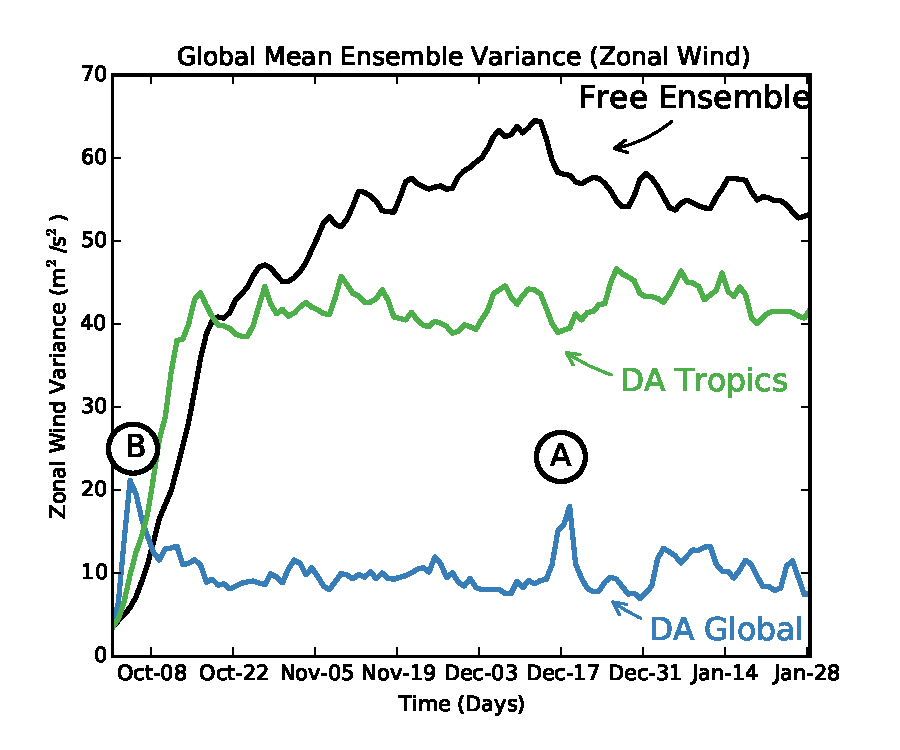
\includegraphics[width=\textwidth]{Paper_figures/ERPDA_paper_evalvariable_state_space.pdf}
	 \caption{Global-average ensemble variance in the zonal wind as a function of time, comparing a DART-WACCM with no assimilation, and with 6-hourly assimilation of meteorolgical observations (see text).}
	 \label{fig:evalvariable_state}
\end{figure}

%-------comparison of the WACCM experiments in terms of aam ----
\begin{figure}
	 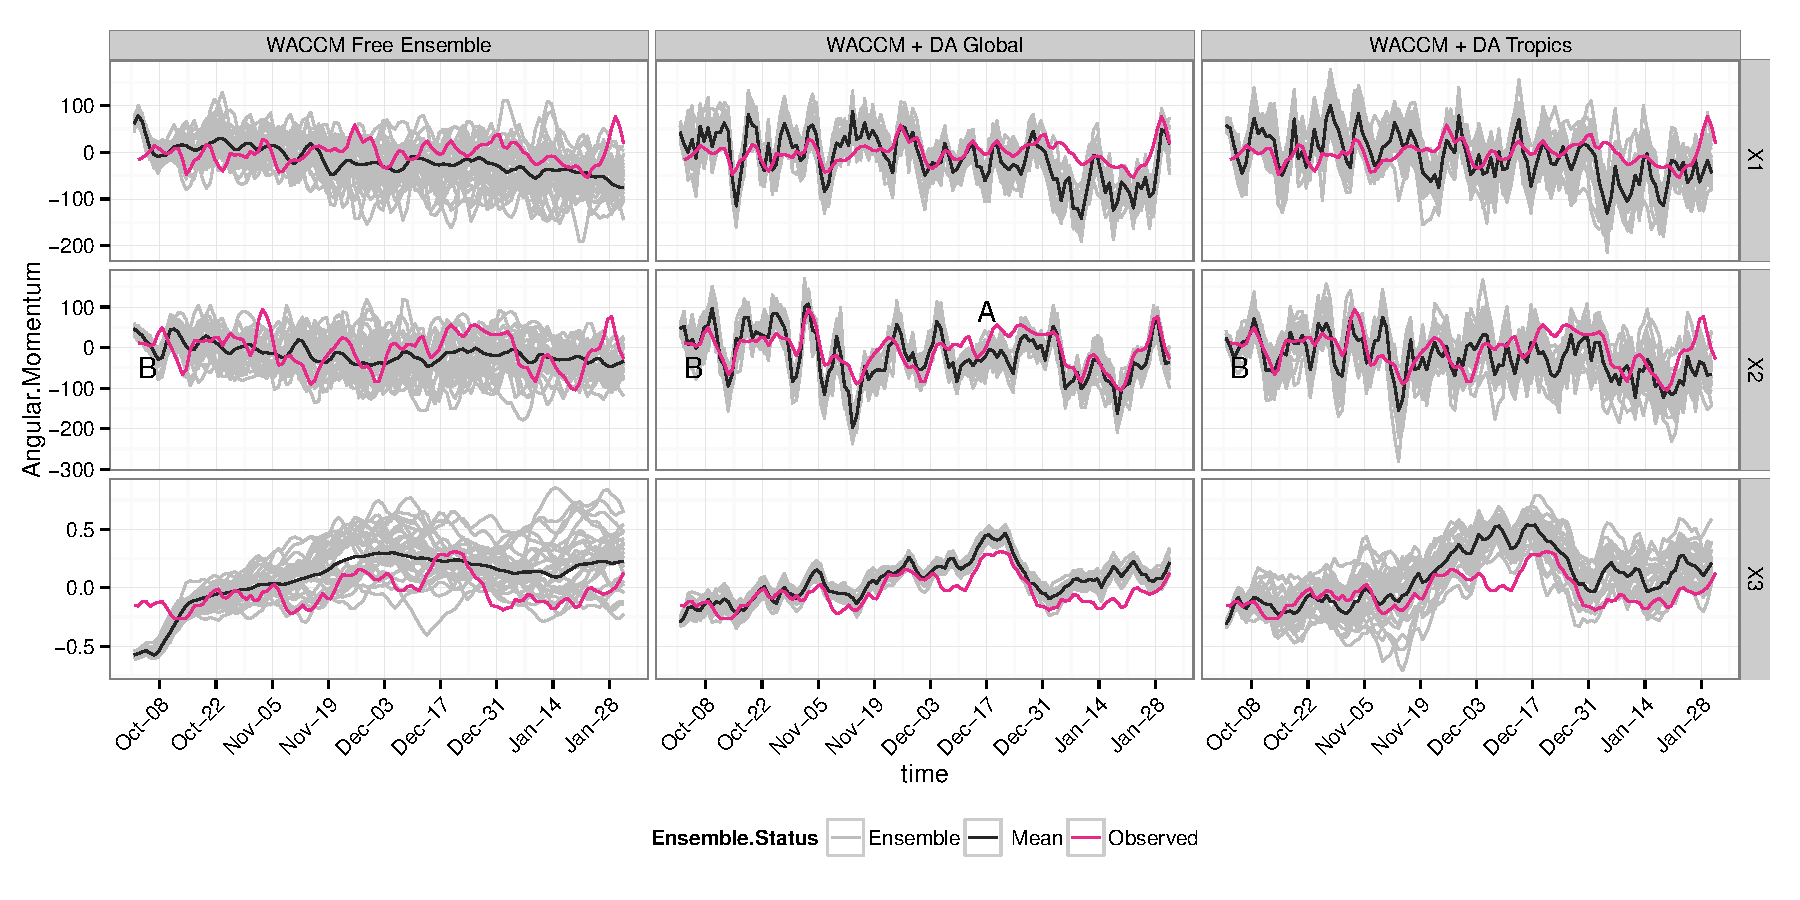
\includegraphics[width=\textwidth]{Paper_figures/ERPDA_paper_evalvariable_aam_space.pdf}
	 \caption{Comparison of the ensemble (gray) and its mean (black) in DART-WACCM experiments with increasing observational constraints (Table \ref{tab:expts}), in terms of angular momentum excitation functions $\chi_2$ and $\chi_3$ Each angular momentum function is compared to the angular momentum implied by the corresponding Earth rotation parameters (pink).}
	 \label{fig:evalvariable_aam}
\end{figure}

%------comparison of the DA runs in the observation space
\begin{figure}[p]
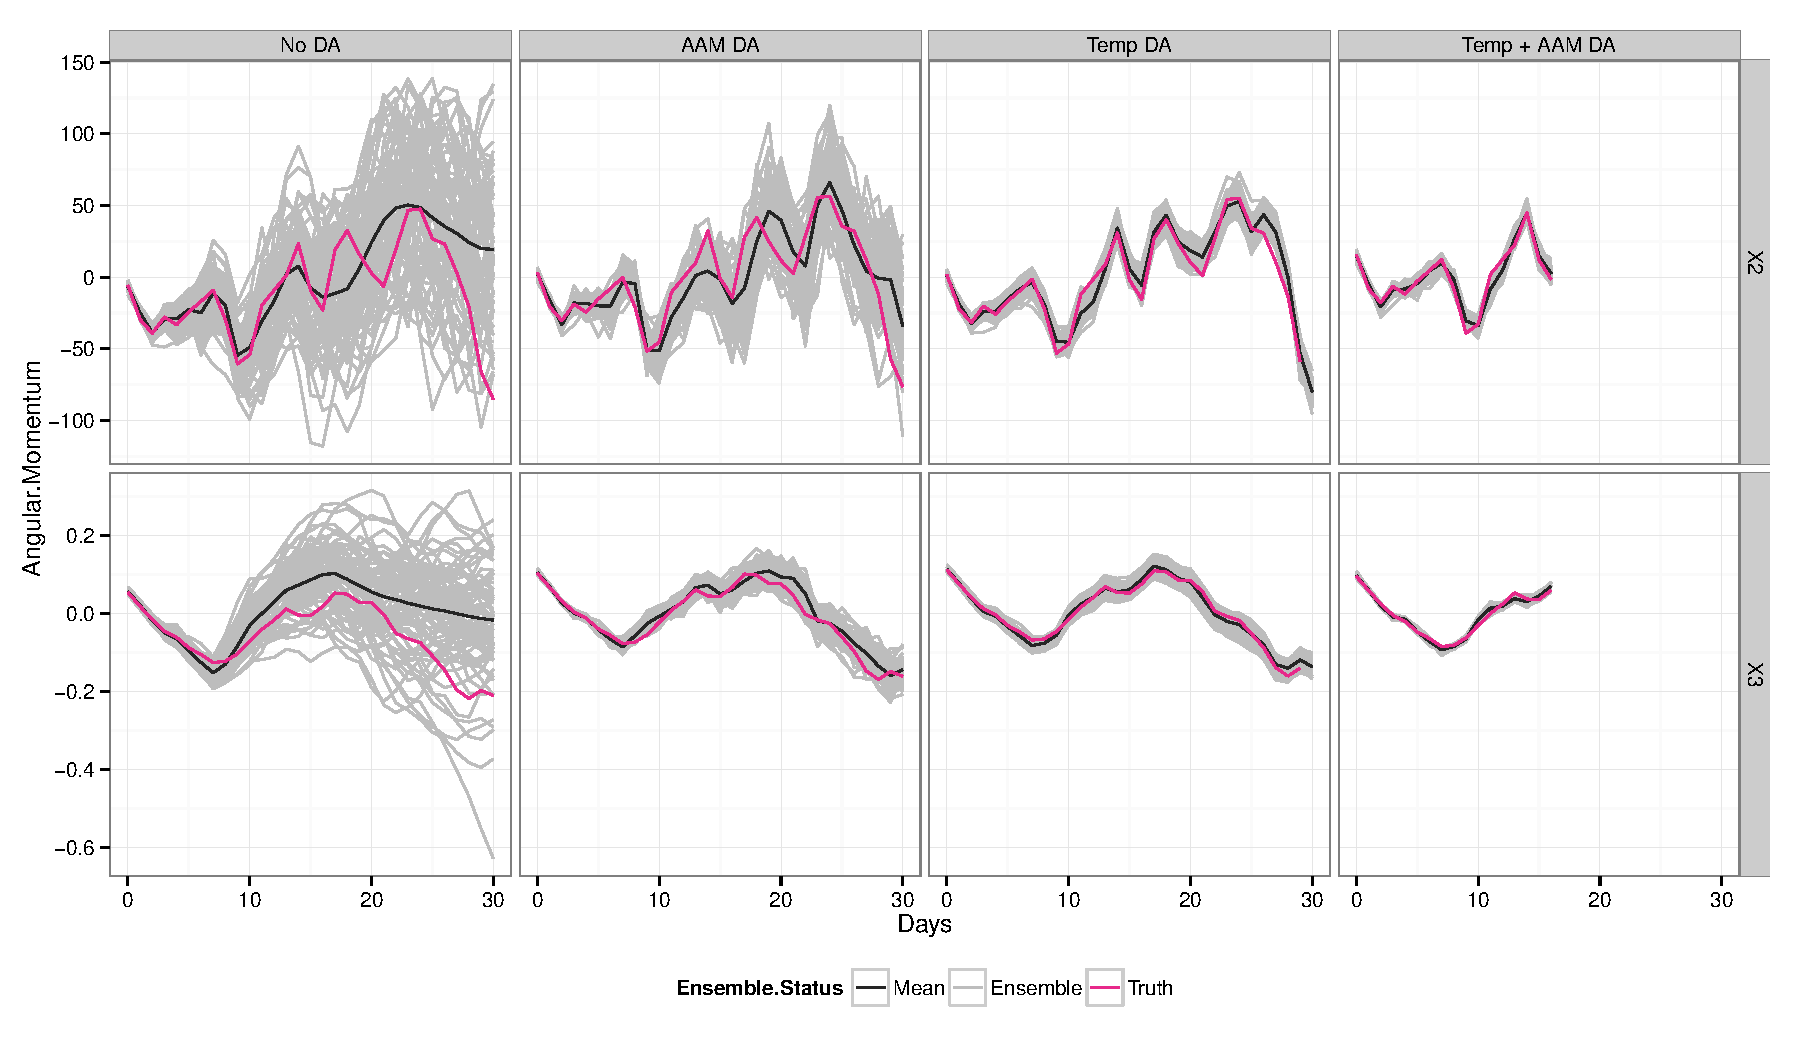
\includegraphics[width=\textwidth]{Paper_figures/ERPDA_paper_erpda_obs_space.pdf} 
\caption{ The DART-CAM prior ensemble (gray) and its mean (black) compared to the true state (pink) in terms of angular momentum components $\chi_2$ and $\chi_3$, comparing four perfect-model experiments with DART-CAM (see text and Table \ref{tab:expts}).  }
 \label{fig:fit_to_ERPs}
\end{figure}

%-----evolution of the covariances between local variables and the AAM observations 
 \begin{figure}
	 \includegraphics[width=\textwidth]{Paper_figures/ERPDA_paper_U_to_LOD_covariances.pdf}
	 \caption{Evolution of the covariance between the zonal wind and the axial angular momentum ($\chi_3$) on three dates, when we assimilate only the three components of angular momentum. The top row shows values averaged over stratospheric levels, while the bottom row shows values averaged over tropospheric levels.}
 \label{fig:covariances}
\end{figure}

%-----evolution of the prior error and corresponding increments 
 \begin{figure}
	 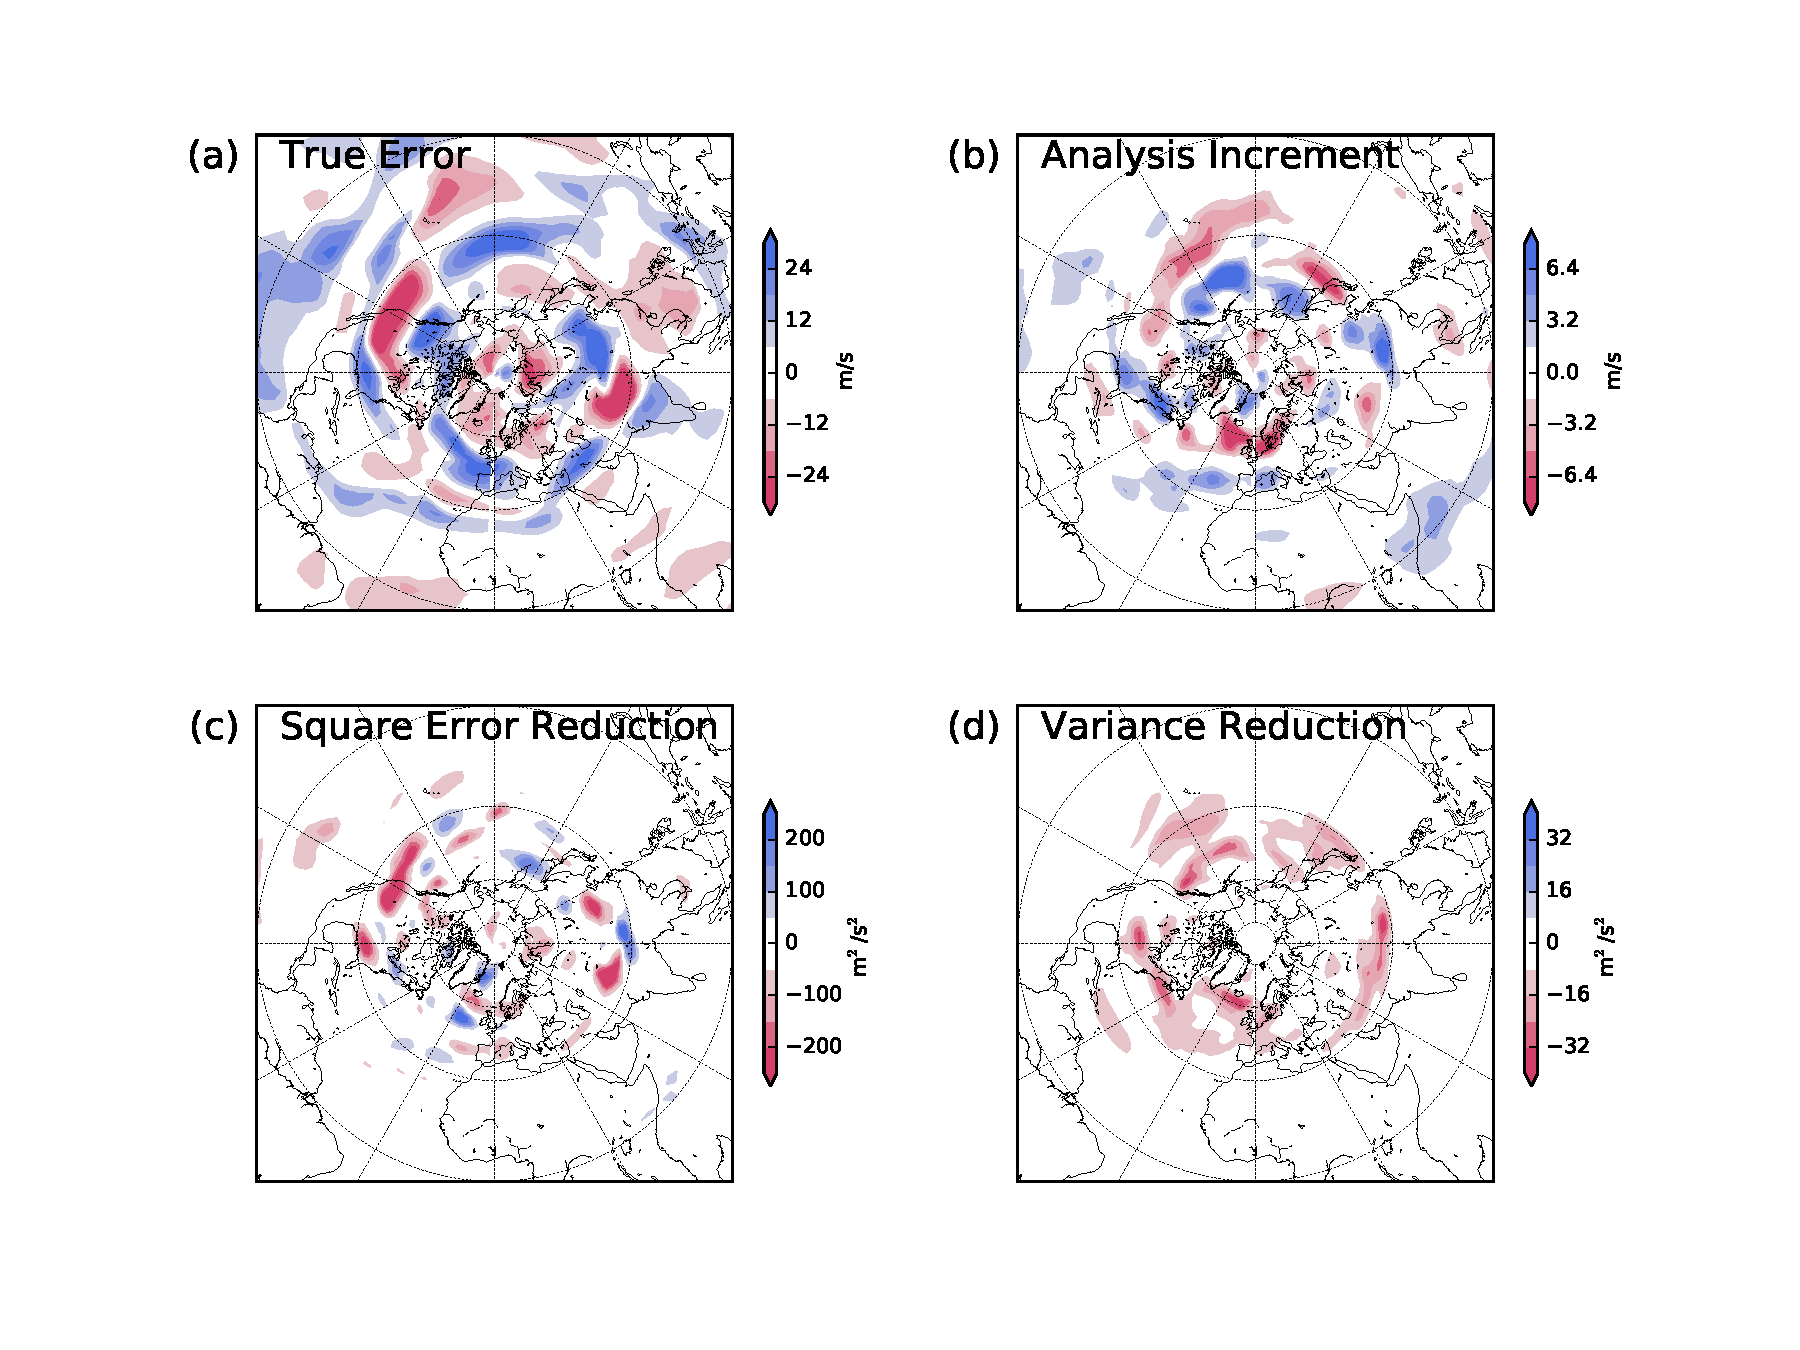
\includegraphics[width=\textwidth]{Paper_figures/ERPDA_paper_U_priorerror_vs_increment_vs_ER_30jan.pdf}
	 \caption{Snapshots of the 320 hPa zonal wind (a) bias (truth minus prior ensemble mean), (b) analysis increment (posterior minus prior ensemble mean), (c) posterior minus prior mean square error, and (d) posterior minus prior ensemble variance on 30 January, assimilating the three angular momentum components only. } 
 \label{fig:error_increments}
\end{figure}


%-----focus on the ensemble in two regions to show how it is moved away from the true state
 \begin{figure}
	 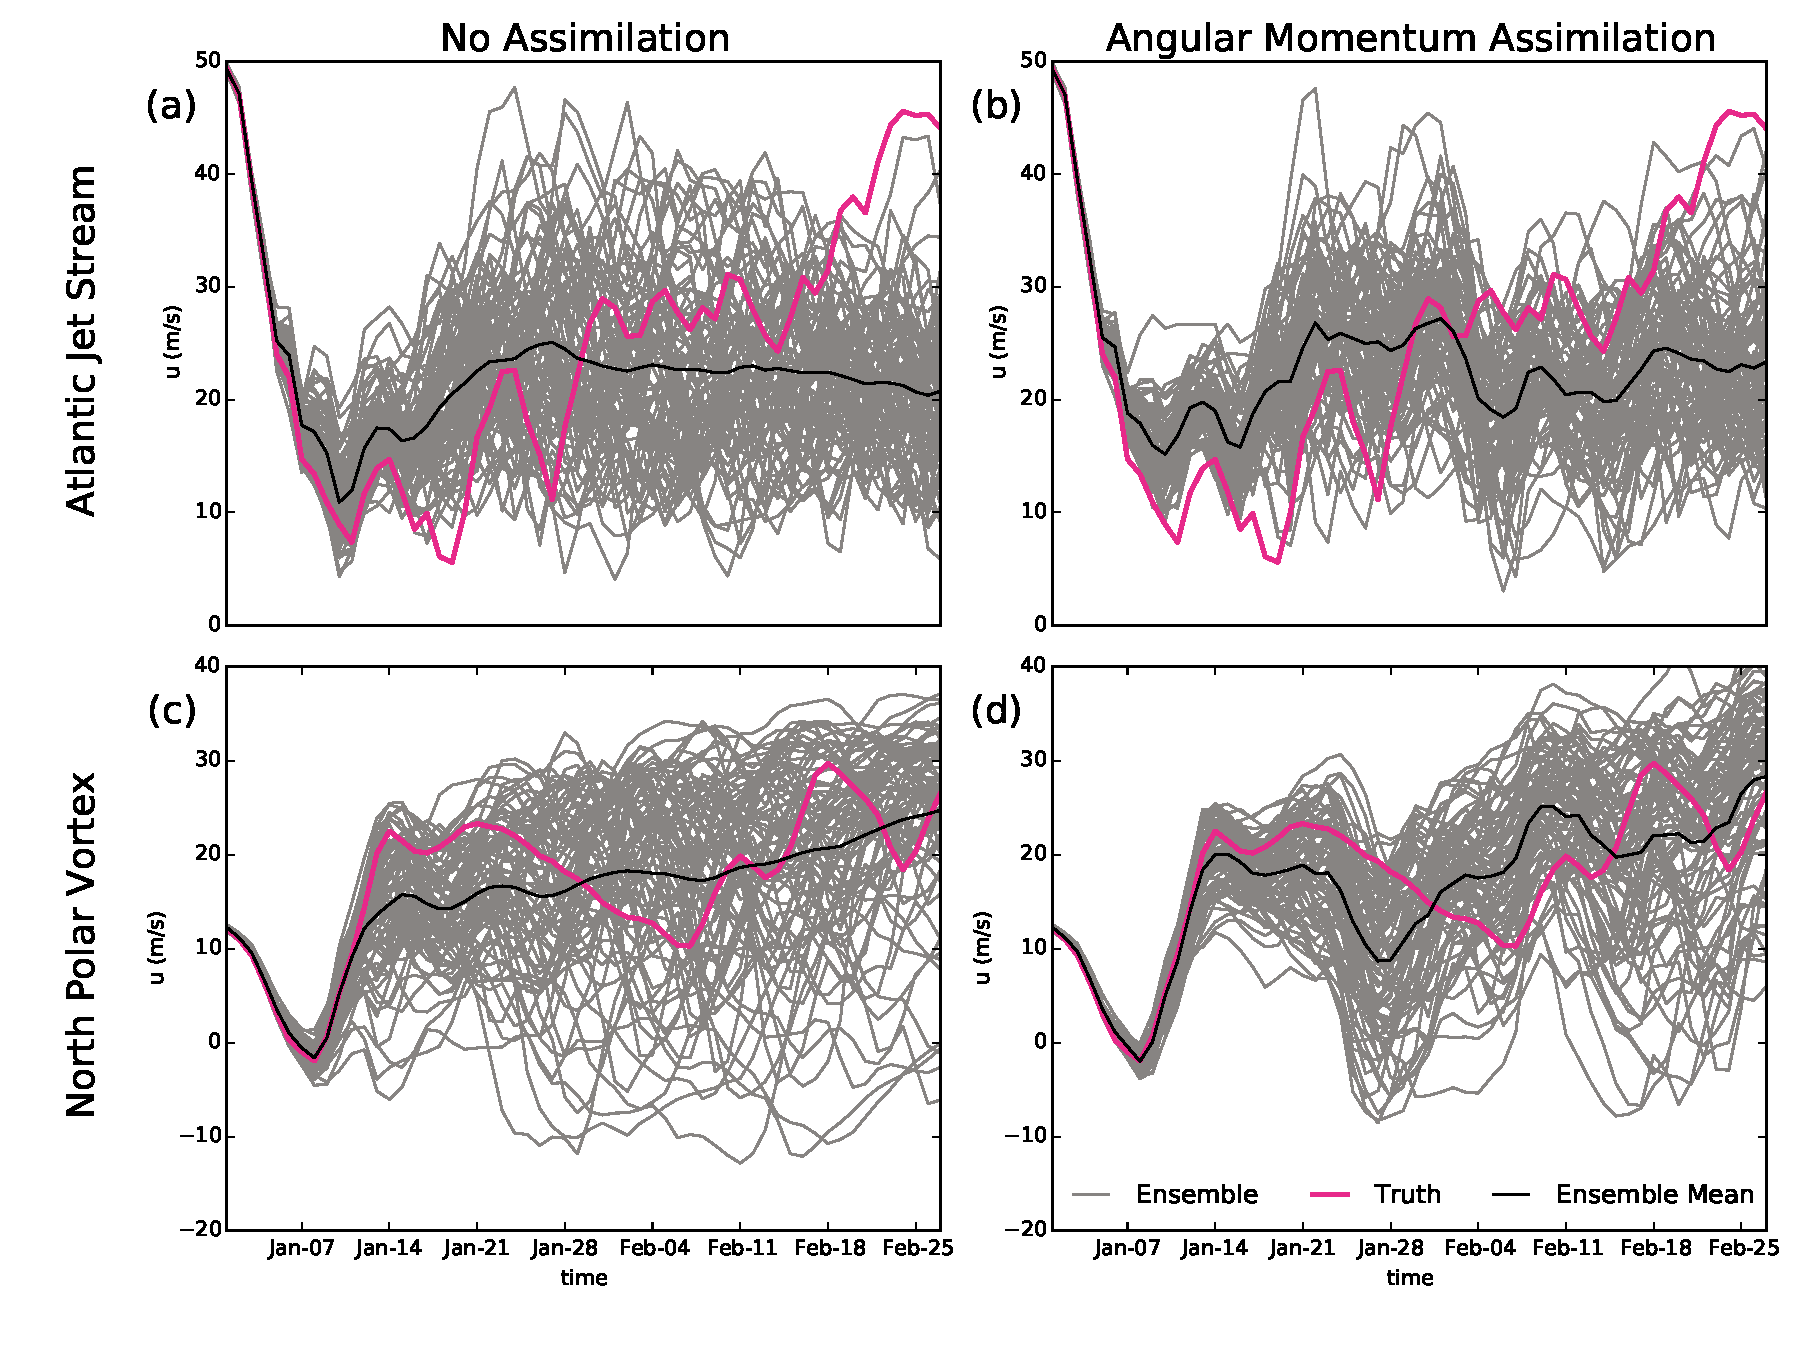
\includegraphics[width=\textwidth]{Paper_figures/ERPDA_paper_point_checks.pdf}
	 \caption{Comparison of the ensemble and its mean to the true state, comparing no assimilation (left column), and assimilation of the three angular momentum components (right column). The top row shows zonal wind averaged over the Atlantic jet stream, and the bottom row shows zonal wind averaged in the polar vortex (see text).}
	 \label{fig:point_checks}
\end{figure}


%------MSE diff between ERPRST and RST (red is good)
 \begin{figure}
	 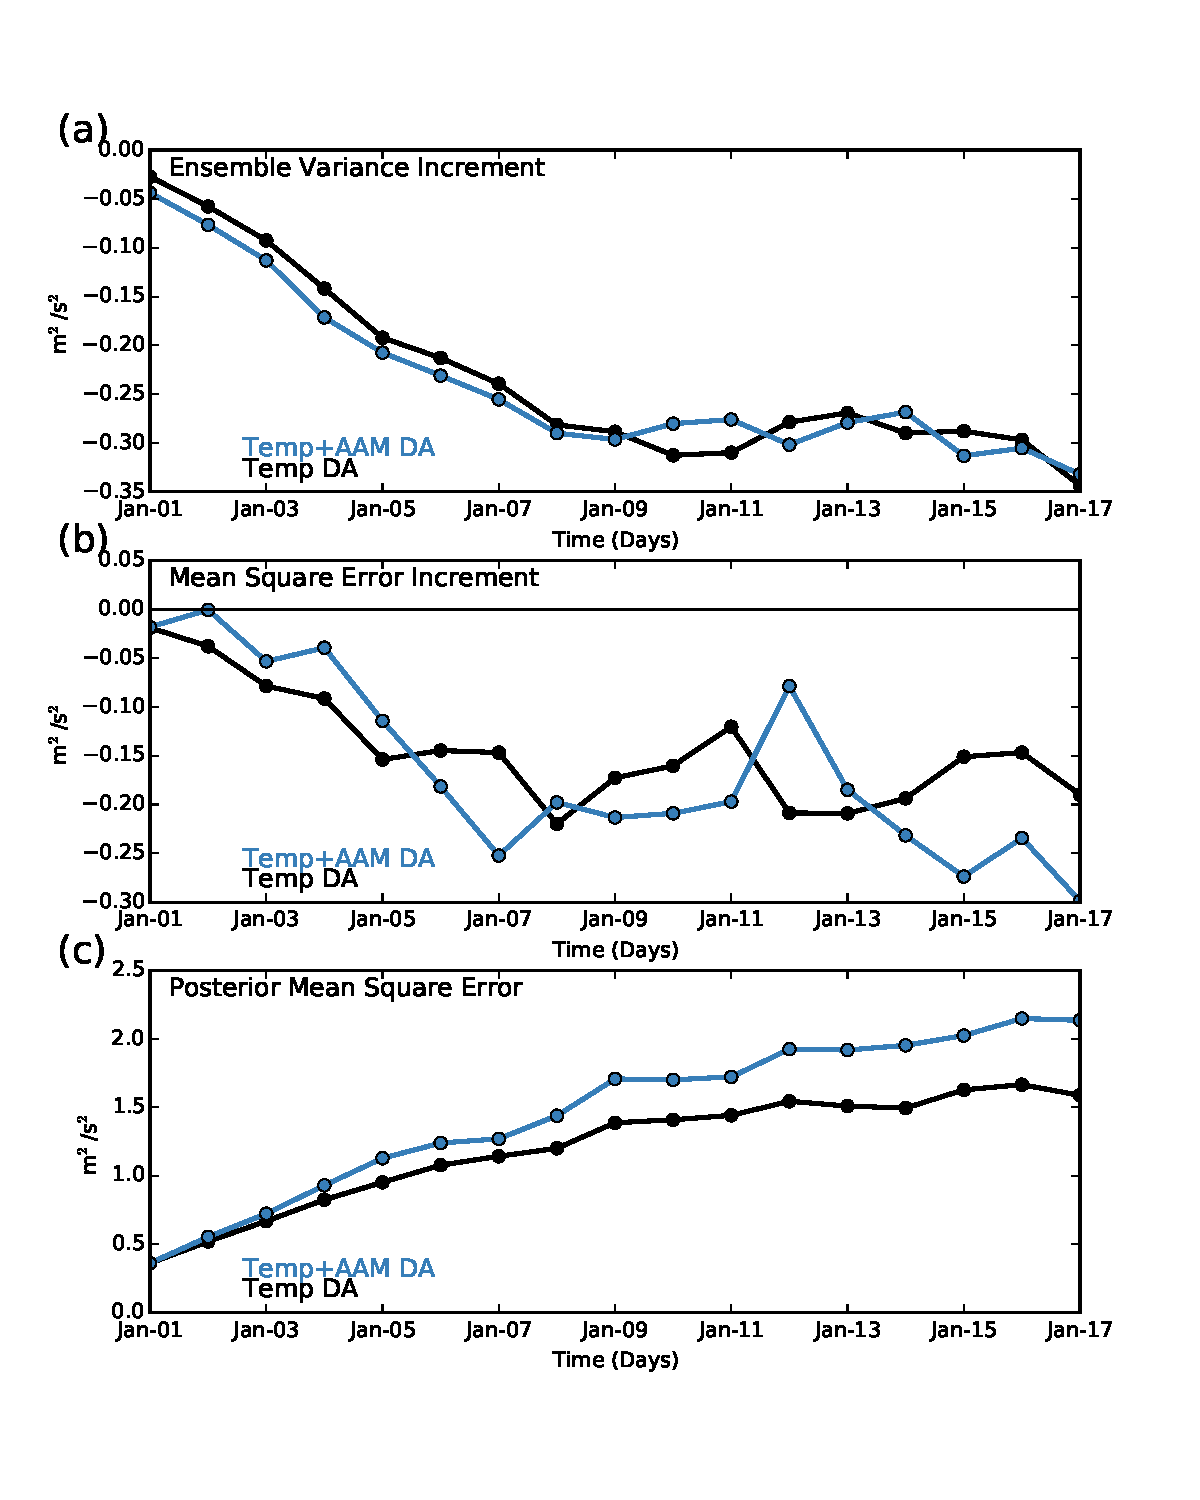
\includegraphics[width=0.7\textwidth]{Paper_figures/ERPDA_paper_MSE_RST_vs_ERPRST_global.pdf}
	 \caption{(a) Global average mean square error (solid lines) and scaled ensemble variance (dashed lines, see eqn \ref{eq:EvsS}) in the surface pressure, comparing the assimilation of regularly-spaced temperature observations with and without additional angular momentum observatins (black and blue, respectively).}
	 \label{fig:added_value_MSE}
\end{figure}
